\section{Dokumentation der Implementierung}

%%%%%%%%%%%%%%%%%%%%%%%%%%%%%%%%%%%%%%%%%%%%%%%%%%
% Abschnitt - Grober Überblick
%%%%%%%%%%%%%%%%%%%%%%%%%%%%%%%%%%%%%%%%%%%%%%%%%%

\subsection{Überblick}

% TODO Ein bisschen mehr details
Das Problem fordert eine Unterteilung in drei wesentliche Bausteine, wie sie in \autoref{fig:architekturuebersicht} zu sehen sind
Eine Benutzeroberfläche in einem Web Browser des Benutzers (“Frontend”), welches die Benutzerinteraktionen entgegennimmt und mit dem Backend kommuniziert.
Ein Backend-Host übernimmt dazu die Kommunikationsfunktion, verwaltet die eingehenden Rechenaufträge und verteilt sie an die Backend-Worker. Das Ergebnis dieser Berechnung sendet der Host dann an das Frontend zurück.
Die Backend-Worker nehmen die zugewiesenen Rechenaufträge entgegen und führen die eigentlichen Berechnungen verteilt aus.

\subsubsection{Frontend}

Das Design der Weboberfläche ist schlicht und modern gehalten und fokussiert sich im wesentlichen auf die Visualisierung der Mandelbrotmenge. Um jedoch weiterhin die vorgenommene Balancierung und den damit resultierenden Einfluss auf die Rechenzeit der einzelnen Bereiche darzustellen werden weitere Diagramme am unteren Rand des Fensters eingeblendet. Dabei ist es immer die oberste Priorität, dem Benutzer möglichst einfach den Effekt unterschiedlicher Lastbalancierungs-strategien für die paralelle Berechnung der Mandelbrotmenge zu präsentieren.

Die Anordnung der Komponenten in unserem Design ist logisch nach Fluss und Erzeugung der Informationen sortiert. Deshalb befinden sich von links nach rechts gelesen in dem unteren Banner Auswahl des Lastbalancieres, Netzwerkdarstellung mit Frontend links über Host zu den Workern, absolute Wartezeiten der Worker und eine relative Darstellung der Rechenzeit.

Die Auswahl des Balancers ist als Liste gestaltet, welche die Auswahl eines der verfügbaren Lastbalancierers erlaubt. Sobald der Benutzer länger die Maus über einen der Einträge hält, wird zusätzlich noch eine Beschreibung über die Funktionalität des Lastbalancierers angezeigt.

Der Systemaufbau wird mit einem Graph visualisiert, dessen Knoten die am System beteiligten, unabhängigen Komponenten (Frontend, Host, Worker) darstellen. Eine Kante bedeutet eine Kommunikationsverbindung zwischen den Komponenten. 

\begin{figure}
    \centering
        % TODO ref einfügen - ohne ref wird das bild nicht benötigt!
        % Wird sich vermutlich noch ändern
        \caption{Visualisierung des Systemaufbaus}
    \label{fig:visualisierung_systemaufbau}
\end{figure}

Das Ziel einer optimalen Lastbalancierung ist es, den gesamten sichtbaren Bereich der Mandelbrotmenge möglichst gleich bezüglich des Rechenaufwandes zwischen den Workern aufzuteilen. Bei einer solchen optimalen Aufteilung werden somit auch die entstehenden Wartezeiten der Worker (Idle Times) minimiert. Diese Wartezeiten werden in dem Balkendiagramm der Idle Time dargestellt. Eine möglichst gute Aufteilung zeigt deshalb eine kleine Gesamtwartezeit aller beteiligten Worker.

\begin{figure}
    \centering
        % TODO ref einfügen - ohne ref wird das bild nicht benötigt!
        % Wird sich vermutlich noch ändern
        \caption{Wartezeiten der Worker}
    \label{fig:visualisierung_wartezeiten_worker}
\end{figure}

In der absoluten Wartezeit werden immer alle Worker außer demjenigen dargestellt, welcher zuletzt fertig wird, da dieser keine Wartezeit erzeugt. Um auch einen relativen Vergleich der Rechenzeiten der Worker darzustellen, ist ebenfalls ein Kuchendiagramm eingebunden, welches die Rechenzeit aller Worker im Verhältnis zueinander darstellt. Eine möglichst gute Aufteilung teilt die Rechenzeit möglichst gleich auf, wodurch die farbigen Flächen im Kuchendiagramm der einzelnen Worker möglichst gleich groß werden.

\begin{figure}
    \centering
        % TODO ref einfügen - ohne ref wird das bild nicht benötigt!
        % Wird sich vermutlich noch ändern
        \caption{Relative Rechenzeiten der Worker}
    \label{fig:visualisierung_relative_rechenzeiten_worker}
\end{figure}

Um ebenfalls darzustellen, welcher Worker, einen gegebenen Teil des sichtbaren Ausschnitts der Mandelbrotmenge berechnet hat, wird ein Overlay eingeführt. Dieses wird halbtransparent über der Visualisierung der Mandelbrotmenge selbst angezeigt und färbt alle disjunkten Bereiche des Lastbalancierers in einer eigenen Farbe ein. Damit zeigt dieses Overlay ebenfalls exakt die Aufteilung, welche der ausgewählte Lastbalancierer bestimmt hat und die vom Backend parallel berechnet wurde. Förderlich ist dies für das Design Ziel des Frontends, da damit dem Benutzer dargestellt werden kann, welche Bereiche der Mandelbrotmenge rechenintensiv darzustellen sind und deshalb mehr Zeit benötigen.

\begin{figure}
    \centering
        % TODO ref einfügen - ohne ref wird das bild nicht benötigt!
        % Wird sich vermutlich noch ändern
        \caption{Overlay einer Lastbalanceriung}
    \label{fig:visualisierung_lastbalancierung}
\end{figure}

Um der Nutzerin eine Zuordnung zwischen Region, Name, Wartezeit und Rechenzeit zu ermöglichen, erhalten in jeder der Komponenten die Knoten jeweils die gleiche Farbe. Die Bereitstellung der entsprechenden Information wird über ein Objekt der Klasse WorkerContext bereitgestellt, welches ebenfalls synchronisiert, welcher der Knoten aktuell im Fokus der Nutzerin steht. Diese Synchronisation wird ebenfalls durch das Observer-Pattern durchgeführt.

\subsubsection{Backend}

Um die Mandelbrotmenge parallel zu berechnen, werden mehrere Worker-Prozesse per MPI auf unterschiedlichen Rechenknoten gestartet. Jeder davon soll jeweils einen Teil der zu berechnenden Region erhalten. Um diese Aufteilung zu koordinieren existiert ein zentraler Host-Prozess. Er teilt sich mit einem der Worker-Prozesse einen Rechenknoten, verteilt Aufgaben an die Worker und nimmt Rechenergebnisse entgegen. Dieser Host-Prozess ist außerdem die zentrale Kommunikationseinheit für das Frontend. Dort findet also die Behandlung der Anfragen und das Versenden der berechneten Regionen an die Benutzeroberfläche statt.

Die Aufgabe des Hosts ist, zunächst Anfragen des Frontends für die komplette Region via Websocket entgegenzunehmen und in Teilregionen aufzuteilen (siehe Lastbalancierung). Die Teilregionen werden anschließend vom Host per MPI an die Worker verteilt, wobei jedem Worker genau eine Teilregion zugeteilt wird (siehe Kommunikation mittels MPI).

Nachdem alle Worker ihre Teilregion erhalten haben, wird die bestimmte Aufteilung vom Host per Websocket an das Frontend weitergeleitet. Dies ist für eine Visualisierung der Aufteilung zwingend nötig.

Nach dem Empfangen einer einzelnen Region beginnen die Worker mit der Berechnung des Bereiches. Dazu wird jeder Pixel auf einen entsprechenden Punkt in der komplexen Ebene projiziert. Die tatsächliche Berechnung des Fraktals für einen Pixel an eine Instanz einer Unterklasse von Fractal delegiert. Da die Bindung an eine konkrete Unterklasse dynamisch geschieht, kann der Fraktaltyp zur Laufzeit gewechselt werden. Der Worker iteriert so über alle Pixel und erstellt ein Ergebnisarray.

Sobald die Berechnungen eines Workers abgeschlossen sind, werden die Ergebnisse wieder mittels MPI an den Host übermittelt.

Damit der Zeitunterschied (vor allem bzgl. der Option ohne Lastbalancierung) bei der Berechnung der verschiedenen Teilregionen für den Nutzer zu sehen ist, müssen die Ergebnisse der Teilregionen mit möglichst geringer Verzögerung vom Backend-Host an das Frontend weitergeleitet werden. Dies wird durch die Verwendung von Websockets ermöglicht.

\begin{figure}
    % Bindet das als PDF exportierte pptx ein -> vektorgrafik
    % -> pptx bearbeiten statt pdf
    \centering
        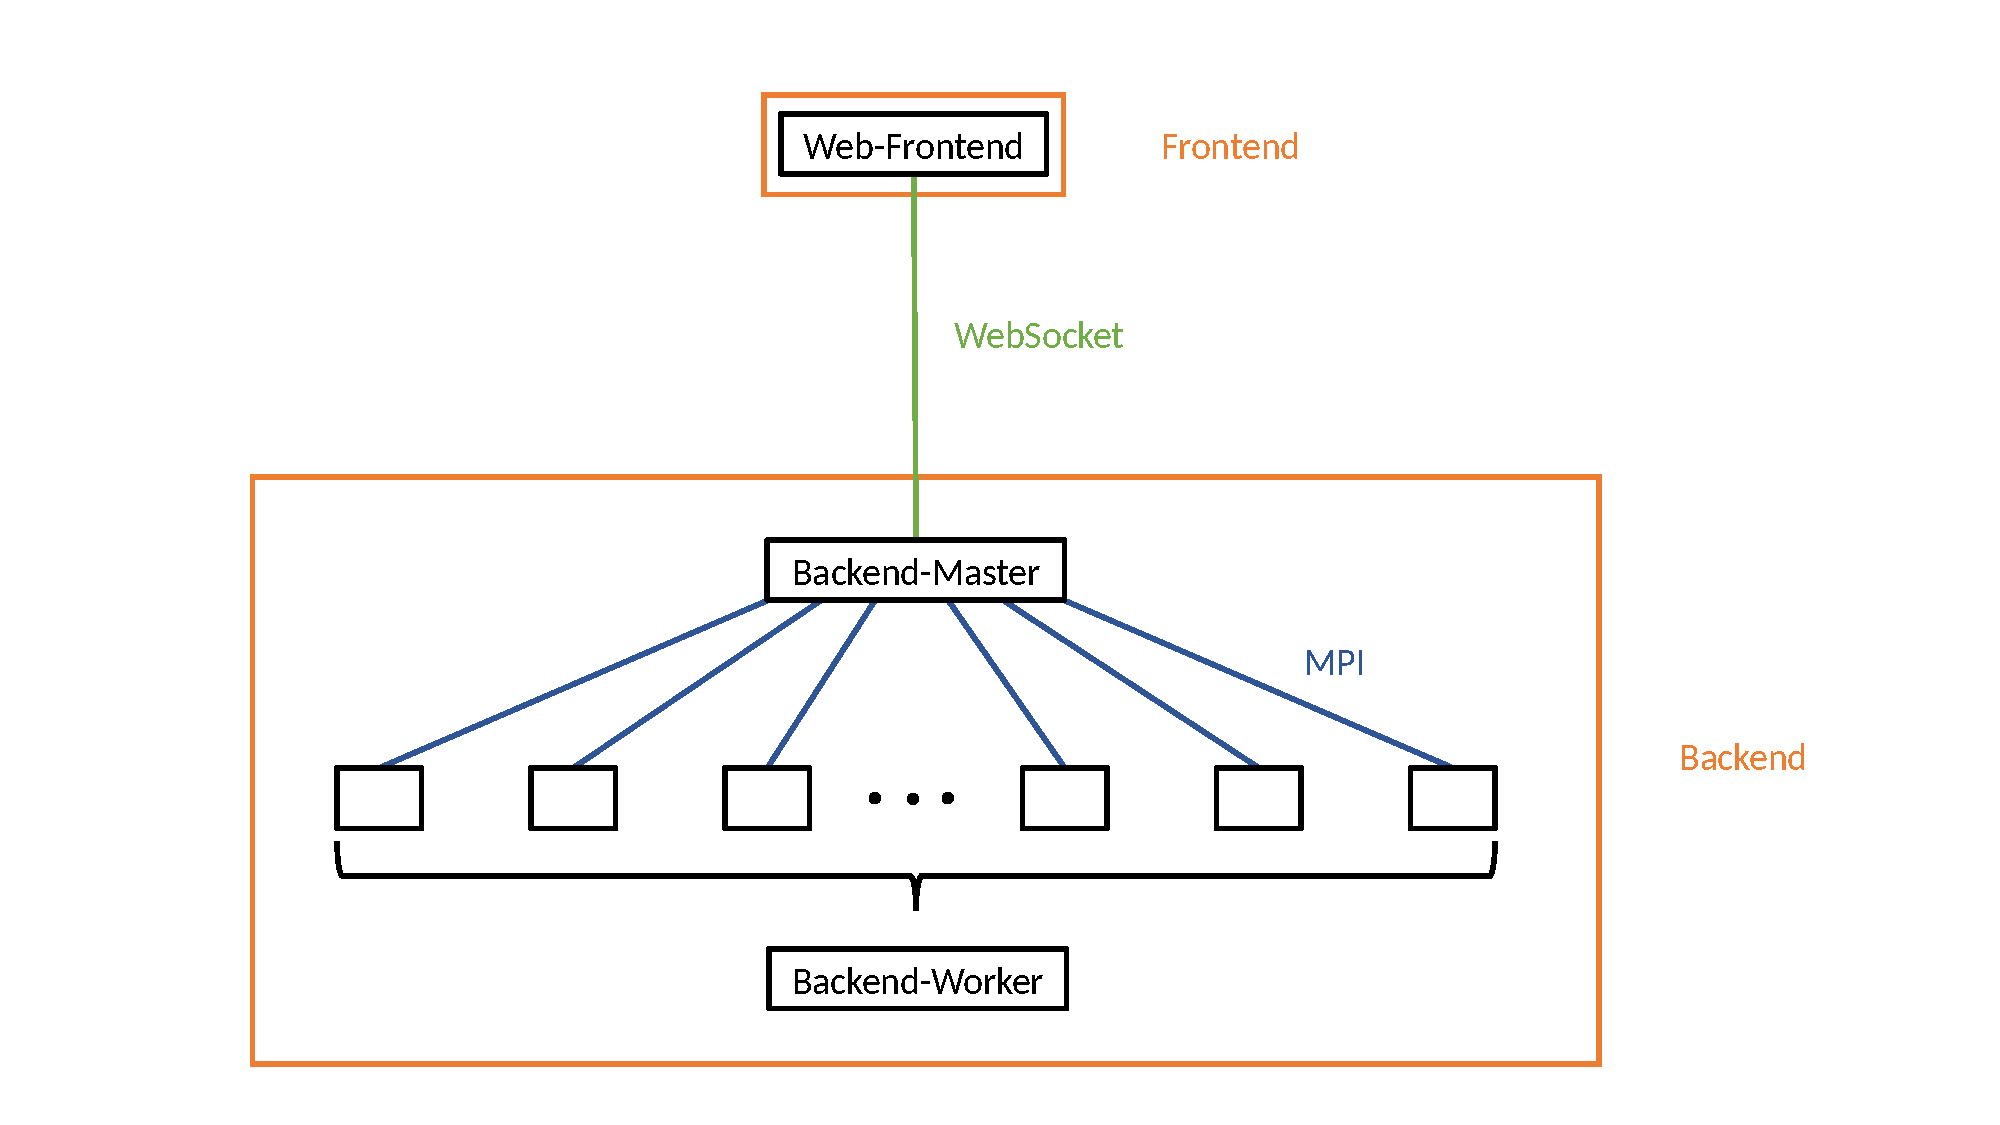
\includegraphics[width=0.98\linewidth]{img/Implementierung/Kommunikation.pdf}
        \caption{Architekturübersicht}
    \label{fig:architekturuebersicht}
\end{figure}

\subsubsection{Lastbalancierung}

Ziel der Lastbalancierung ist es, die Rechenlast so gut wie möglich auf die zur Verfügung stehenden Rechenkerne aufzuteilen. Hierzu wird die Region in Teilregionen aufgeteilt.

Es stehen momentan eine naive Strategie und eine Strategie mit Vorhersage zur Verfügung.

Die naive Strategie (Naive Balancer) teilt die Region in möglichst gleich große Teilregionen auf. Da dies ohne Rücksicht auf eventuell unterschiedliche Rechenzeiten in den einzelnen Teilregionen geschieht, kann es dabei zu einer schlechten Lastverteilung kommen.

\begin{figure}
    \centering
        % TODO include image
        % TODO ref auf das image im text, sonst ist es nutzlos!
        \caption{Naive Strategie zur Lastbalancierung}
    \label{fig:lastbalanceriung_naiv}
\end{figure}

Bei der Strategie mit Vorhersage (Prediction Balancer) wird die zu berechnende Region vor der Aufteilung in geringerer Auflösung im Host vorberechnet. Die Teilregionen werden dann so gewählt, dass der durch die Vorhersage abgeschätzte Rechenaufwand möglichst gleich unter den Workern verteilt ist. Aber auch diese Strategie ist nicht perfekt. Die Vorhersage ist durch die geringere Auflösung vor allem am Rand des Fraktals ungenau. Die Genauigkeit der Vorhersage zu erhöhen bedeutet zusätzlichen Rechenaufwand während der Balancierung. Dieser sollte in einem sinnvollen Verhältnis zum Aufwand der Berechnung des Fraktals stehen. Einen perfekten Ausgleich zu finden ist wesentliche Aufgabe ernsthafter Optimierungsansätze.

\begin{figure}
    \centering
        % TODO include image
        % TODO ref auf das image im text, sonst ist es nutzlos!
        \caption{Strategie mit Vorhersage zur Lastbalancierung}
    \label{fig:lastbalanceriung_vorhersage}
\end{figure}

%%%%%%%%%%%%%%%%%%%%%%%%%%%%%%%%%%%%%%%%%%%%%%%%%%
% Abschnitt - wie läuft das auf meinem System?
%%%%%%%%%%%%%%%%%%%%%%%%%%%%%%%%%%%%%%%%%%%%%%%%%%

\subsection{Installation}

\subsubsection{Frontend}

% TODO notwendig? Vllt noch zuvor erklären dass/wie alles benötigte installiert wird (npm)
Um das Frontend zu implementieren, wurde sich für die Programmiersprache JavaScript (ECMAScript 6 Standard\footnote{\url{https://www.ecma-international.org/publications/standards/Ecma-262.htm}}) entschieden. Diese erlaubt uns, Berechnungen innerhalb des Browsers auszuführen und erlaubt gestalterische Freiheit. Zudem wird ermöglicht dynamisch auf Eingaben des Nutzers zu reagieren.

Moderne Browser verwenden zum Anzeigen von Webseiten HTML (Hyper-Text-Markup-Language) Code, welcher die hierarchische Struktur einer Seite definiert und CSS (Cascading-Style-Sheets), um diese zu layouten. Um den benötigten HTML Code dynamisch in Reaktion auf eine Eingabe des Benutzers verändern zu können wird das React Framework\footnote{\url{https://reactjs.org/}} verwendet. Dieses erlaubt für jede logische Komponente eine eigene JavaScript Klasse zu erstellen, welche dann den betreffenden HTML Code generiert. Somit wird eine logische Trennung der einzelnen Domänen der Frontend Applikation erreicht, wodurch die Wartbarkeit des Systems erhöht wird.

Um das Fraktal darzustellen wird die Leaflet Bibliothek\footnote{\url{http://leafletjs.com/}} verwendet. Diese, eigentlich für Onlinekarten konzipierte, Bibliothek stellt einen Bereich der komplexen Ebene, auf der die Mandelbrotmenge liegt, dar. Diese sichtbare Region wird dann an das Backend versendet und vom Lastbalancierer  in Teilregionen aufgeteilt. Die so entstandenen Teilregionen werden im Backend bearbeitet und die resultierenden Daten an das Frontend versendet. Dort wird jede Teilregion in kleine Kacheln von konstanter Größe aufgeteilt. Das nachfolgende Bild zeigt beispielhaft eine solche Aufteilung. Hier sind die Regionen der Lastbalancierung des Backends weiß gestrichelt und die von Leaflet erzeugten Kacheln rot umrandet dargestellt.

Die Leaflet Bibliothek lässt sich einfach in den generierten HTML Code einbinden und weiter für spezifische Features erweitern.
Neben der Visualisierung der Mandelbrotmenge selbst wird ebenfalls die Bibliothek chart.js\footnote{\url{https://www.chartjs.org/}} für Balken- und Kreisdiagramme verwendet.

Weiterhin wird vis.js\footnote{\url{http://visjs.org/}} als Netzwerkgraphenbibliothek verwendet, um den Aufbau des Systems zu visualisieren. 

Damit eine konsistente Version aller verwendeten Libraries über die Lebensdauer des Projekts gewährleistet werden kann, verwenden wir npm\footnote{\url{https://www.npmjs.com/}} als Paketmanager der verwendeten Libraries. Dieses ermöglicht es, genaue Versionen der verwendeten Pakete zu spezifizieren und bietet eine entwicklerfreundliche Kommandozeilenanwendung um Pakete zu installieren und zu aktualisieren.

\subsection{Backend}

% TODO was ist hier wesentlich für die Installation? Sollen Teile hieraus in die Codedoku?

Als Programmiersprache im Backend wird C++ verwendet. Zum einen bietet C++ hochsprachliche Konstrukte, wie die Möglichkeit Objekte in Klassen zu organisieren. Auch Vererbung und Polymorphie, zwei wichtige Konzepte der objektorientierten Programmierung, können genutzt werden, um die Wartung und Erweiterung des Systems zu erleichtern. Zum anderen ist C++ eine vergleichsweise maschinennahe und somit performante Sprache.

Für die Websocket-Verbindung zum Frontend wird die websocketpp Bibliothek\footnote{\url{https://github.com/zaphoyd/websocketpp}} als leichtgewichtige und performante Implementierung eingesetzt.

Die Kommunikation der verschiedenen Prozesse des Backends wird mittels MPI realisiert. Das Message Passing Interface\footnote{\url{https://www.mpi-forum.org/}} ist eine weit verbreitete Spezifikation, die Kommunikation zwischen unabhängigen Rechenkernen regelt. Dadurch existieren viele gut funktionierende Umsetzungen in einer Vielzahl von Programmiersprachen. Durch MPI wird echte Parallelisierung mit geringem Overhead ermöglicht. Es können so die einzelnen Workerprozesse auf jeweils einem eigenen unabhängigen Rechenkernen laufen. Die Gestaltung von MPI erlaubt dabei alle möglichen Aufteilungen, von Kernen auf einem Prozessor bis hin zu unabhängigen Clustern, die lediglich eine SSH-Verbindung besitzen.

% Löschen? Oder ändern zu "wurde getestet auf"?
Als konkrete Implementierung wurde sich für MPICH entschieden. Ein Grund dafür ist, dass MPICH stetig weiterentwickelt und verbessert wird, es also regelmäßig Veröffentlichungen mit neuen Features und Bugfixes gibt. Zudem ist diese Implementierung sehr gut dokumentiert, weit verbreitet und es existiert eine sehr aktive Community mit Blogs und Tutorials. Dies macht es für alle Beteiligten leicht, sich in die Materie einzulesen und kann in Zukunft für eine schnelle und zuverlässige Lösung von Problemen sorgen. Außerdem wird MPICH zusammen mit C++ auf einer Vielzahl von Systemen unterstützt, wozu auch der Raspberry Pi gehört. Da für dieses Projekt nur die allgemein spezifizierten Funktionen von MPI verwendet werden, sollte das Backend aber auch mit allen anderen gängigen MPI-Implementierungen (z.B. OpenMPI) ausführbar sein.


%%%%%%%%%%%%%%%%%%%%%%%%%%%%%%%%%%%%%%%%%%%%%%%%%%
% Abschnitt - Code Dokumentation
%%%%%%%%%%%%%%%%%%%%%%%%%%%%%%%%%%%%%%%%%%%%%%%%%%

\subsection{Technische Spezifikation}

\subsubsection{Frontend}
% TODO Detaillierter, einzelne Funktionen und Klassen erklären
Das Frontend der Applikation ist im Kern als monolithische Applikation realisiert, welche Daten aus dem Backend empfängt und diese dem Benutzer anzeigt. Aus den verschiedenen Aufgabenbereichen der Darstellung ergibt sich eine logische Trennung  der Komponenten, auch im Code. Das System (Window) besteht dabei aus den Komponenten Display, Visualization, Interaction und WebSocket Client.

Durch eine hierarchische Dekomposition besteht das Fenster (Window) unter anderem aus der Display Komponente, welche die verschiedenen Layer der Leaflet Bibliothek enthält. Dieser wird in einen Fraktal Layer, welcher das Fraktal dem Benutzer anzeigt und einen Worker Layer der die Lastbalancierung des Backends darstellt, differenziert. 

Ebenfalls werden die Komponenten Visualization und Interaction erzeugt, welche Diagramme über die relative Verteilung der Rechenzeit, die Netzwerkdarstellung der Kommunikation des verteilten Systems und Komponenten zur Auswahl der Fraktale sowie Lastbalancierer durch den Benutzer enthalten. 

Das Fenster erzeugt dabei initial eine Websocket Verbindung zum Backend, welche durch Anwendung des Observer Patterns den Komponenten des Windows ermöglicht auf empfangene Daten zu reagieren. Dabei registrieren alle beteiligten Objekte einen Callback bei der WebSocket Verbindung, welcher evaluiert wird sobald Daten vorliegen. Dieses Pattern wird auch auf den Austausch der Informationen über den momentan ausgewählten Lastbalancierer und Fraktal angewendet, um eine responsive Anwendung zu ermöglichen.

\begin{itemize}
	\item Sollte größter Teil werden
	\item \begin{enumerate}
		      \item High level overview?
		      \item Wie läuft das auf meinem System?
		      \item Code Dokumentation / Entwicklerdokumentation
	      \end{enumerate}
\end{itemize}

\subsubsection{Backend}

\begin{figure}
    \centering
        % Exportiertes svg -> modifiziere SVG, export nach pdf
        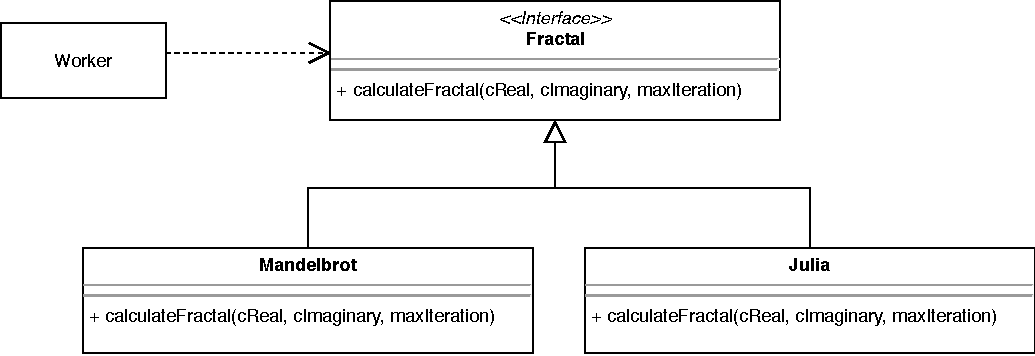
\includegraphics[width=0.8\linewidth]{img/Implementierung/Fractals.pdf}
        \caption{Klassendiagramm für Fractal}
    \label{fig:klassendiagramm_fractal}
\end{figure}